\chapter{Perancangan}
\label{sec:perancangan}

Bab ini membahas mengenai perancangan aplikasi yang akan dibangun meliputi diagram kelas rinci beserta deskripsi dan fungsinya.

\section{Rancangan Kelas Lengkap}
\label{sec:kelaslengkap}
Rancangan kelas dibawah ini akan menampilkan keseluruhan kelas yang akan digunakan. Deskripsi kelas berserta fungsi dari diagram kelas tersebut adalah sebagai berikut:

\begin{figure}[H]
	\centering  
	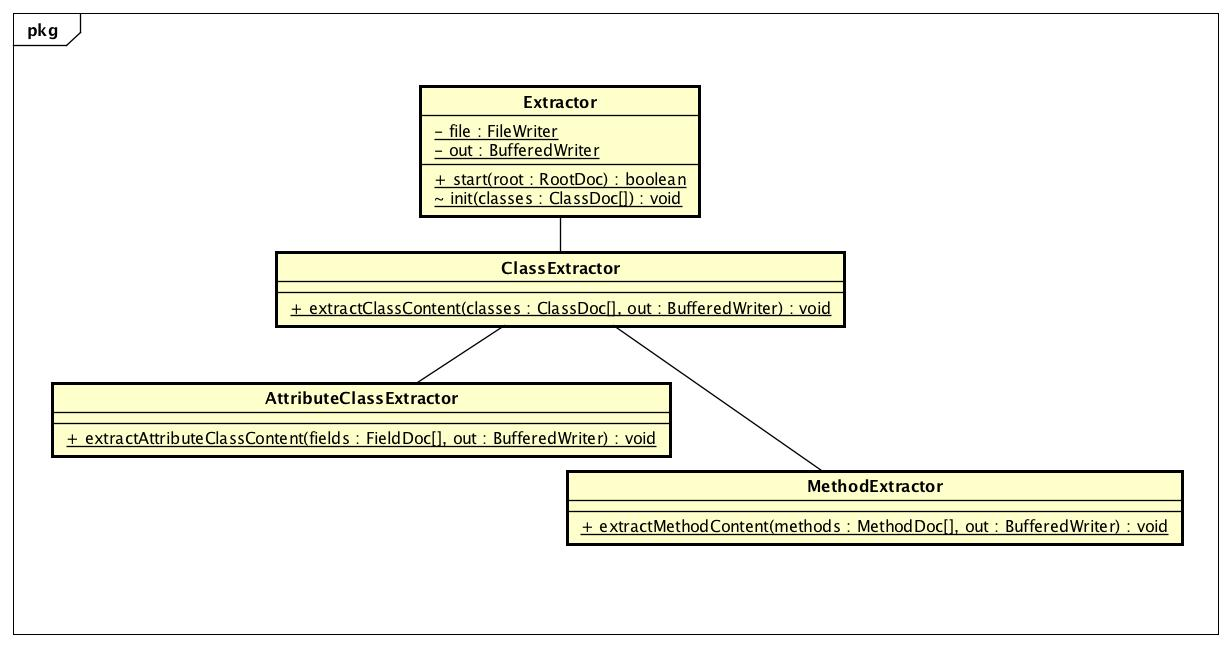
\includegraphics[scale=0.38]{kelas-diagram}  
	\caption[Kelas Diagram]{Kelas Diagram} 
	\label{fig:kelas-diagram} 
\end{figure} 

\begin{enumerate}
	\item {\texttt{ClassExtractor}}\\
	Kelas ini merupakan kelas untuk mengambil informasi sebuah kelas. Atribut yang dimiliki oleh kelas ini adalah sebagai berikut:
	\begin{itemize}
		\item 
	\end{itemize}
	 
	\item {\texttt{AttributeClassExtractor}}\\
	Kelas ini merupakan kelas untuk mengambil informasi sebuah atribut yang terdapat pada kelas. Atribut yang dimiliki oleh kelas ini adalah sebagai berikut:
	\begin{itemize}
		\item 
	\end{itemize}

	
	\item {\texttt{MethodExtractor}}\\
	Kelas ini merupakan kelas untuk mengambil informasi sebuah {\it method} terdapat pada kelas. Atribut yang dimiliki oleh kelas ini adalah sebagai berikut:
	\begin{itemize}
		\item 
	\end{itemize}
	
\end{enumerate}

\section{Rancangan Antarmuka}
\label{sec:antarmuka}
Rancangan antarmuka perangkat lunak yang dibuat adalah melalui sebuah {\it terminal} pada {\it Linux} dan {\it command prompt} pada {\it Windows}. Berikut adalah antarmuka jika menggunakan {\it terminal} pada {\it Linux}: 



